\section{AT mit SimpleKMeans geclustert} \label{SimpleKMeansgeclustert}

In Abbildungen \ref{fig:100Attribute1024ClusterCluster15}, \ref{fig:100Attribute1024ClusterCluster49},  \ref{fig:100Attribute1024ClusterCluster61},  \ref{fig:100Attribute1024ClusterCluster86},  \ref{fig:100Attribute1024ClusterCluster554},  \ref{fig:1000Attribute32ClusterCluster4},  \ref{fig:1000Attribute32ClusterCluster5} sowie \ref{fig:1000Attribute32ClusterCluster6} sind Verse zu sehen, die mit SimpleKMeans in ein Cluster gruppiert wurden.

Bei Abbildung \ref{fig:100Attribute1024ClusterCluster49} auf Seite \pageref{fig:100Attribute1024ClusterCluster49} f�llt auf, dass nicht nur in jedem Vers das Wort Herrn vorkommt, und dass auch alle mit der Versnummer 2 anfangen, sondern auch, dass oft die Formulierung "`Und er tat, was dem Herrn �bel gefiel"' erscheint.

Bei Abbildung \ref{fig:100Attribute1024ClusterCluster554} auf Seite \pageref{fig:100Attribute1024ClusterCluster554} f�llt auf, dass nicht nur in jedem Vers das Wort "`einen"' vorkommt, sondern dass auch alle mit der Versnummer 1 anfangen.

Auf Abbildung \ref{fig:100Attribute1024ClusterCluster86} auf Seite \pageref{fig:100Attribute1024ClusterCluster86} ist zu sehen, dass hier alle Verse vorkommen, die die Formulierung "`Was aber mehr von ... zu sagen ist und was er getan hat, und seine Macht, und wie er..."' beinhalten.

Wenn es eine hohe Anzahl von Attributen gibt, kann der Cluster-Algorithmus viele W�rter erfassen, mit denen Verse sich �hneln k�nnen. Bei vielen �hnlichen Versen brauch der Algorithmus dann aber auch viele Cluster, auf die er die vielen �hnlichen Verse aufteilen kann.

Wenn der Algorithmus nur wenige Attribute aber viele Cluster hat, dann gruppiert er die wenigen Attribute, die ihm zur Verf�gung stehen �ber alle Cluster auf. Wie gut er dabei ist, kann man bei wenigen W�rtern leicht �bersehen, da die meisten W�rter der Verse gar nicht ber�cksichtigt wurden. In den Meisten der 1024 Cluster gibt es aber ein Wort, das alle Verse in diesem Cluster gemeinsam haben.

Es ist zu vermuten, dass wenn alle Attribute genommen werden, die mindestens zwei mal vorkommen, bei steigender Clusteranzahl, die Verse die in einem Cluster vorkommen, zwar im Mittel weniger werden, aber daf�r immer �hnlicher.

\begin{figure}[htp]
\centering
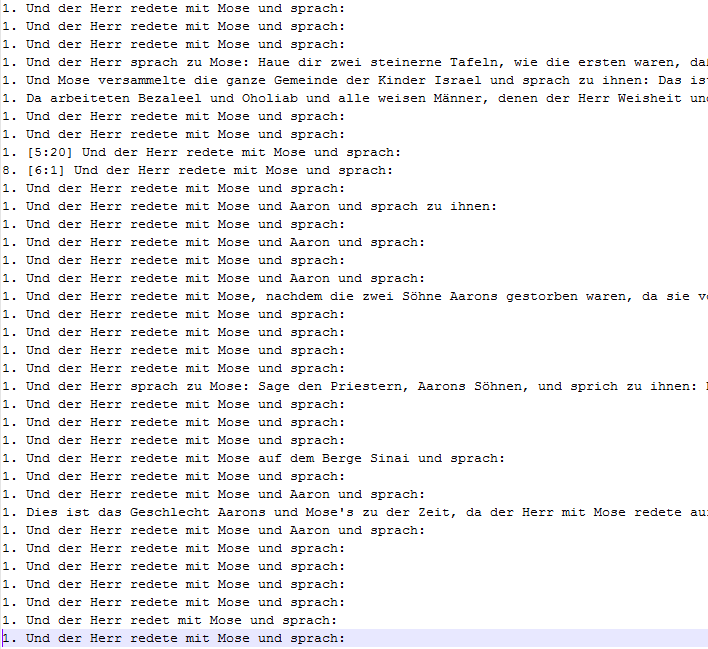
\includegraphics[width=1\textwidth]{Ingo/Bilder/SimpleKMeans100Attr1024Cluster_15.png}
\caption{100 Attribute, 1024 Cluster, Cluster 15}
\label{fig:100Attribute1024ClusterCluster15}
\end{figure}


\begin{figure}[htp]
\centering
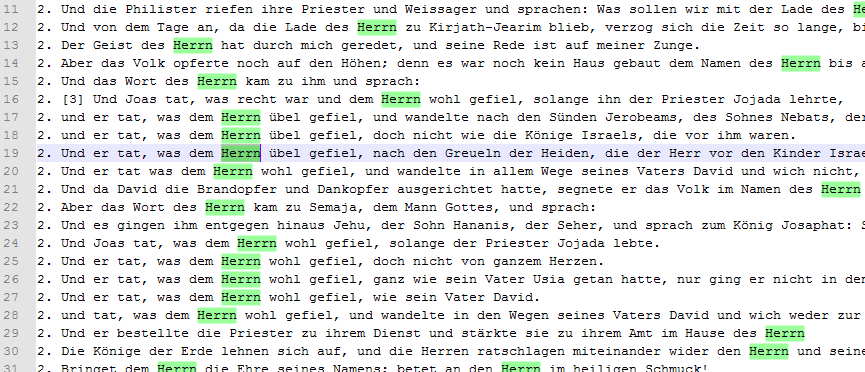
\includegraphics[width=1\textwidth]{Ingo/Bilder/SimpleKMeans100Attr1024Cluster_49.png}
\caption{100 Attribute, 1024 Cluster, Cluster 49}
\label{fig:100Attribute1024ClusterCluster49}
\end{figure}


\begin{figure}[htp]
\centering
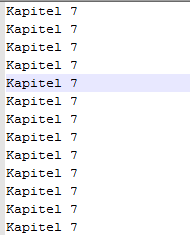
\includegraphics[width=1\textwidth]{Ingo/Bilder/SimpleKMeans100Attr1024Cluster_61.png}
\caption{100 Attribute, 1024 Cluster, Cluster 61}
\label{fig:100Attribute1024ClusterCluster61}
\end{figure}

\begin{figure}[htp]
\centering
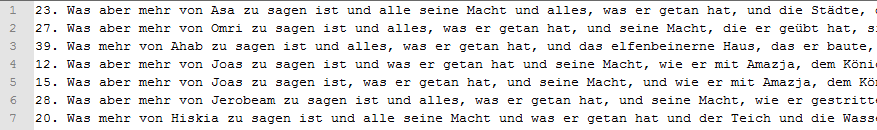
\includegraphics[width=1\textwidth]{Ingo/Bilder/SimpleKMeans100Attr1024Cluster_86.png}
\caption{100 Attribute, 1024 Cluster, Cluster 86}
\label{fig:100Attribute1024ClusterCluster86}
\end{figure}

\begin{figure}[htp]
\centering
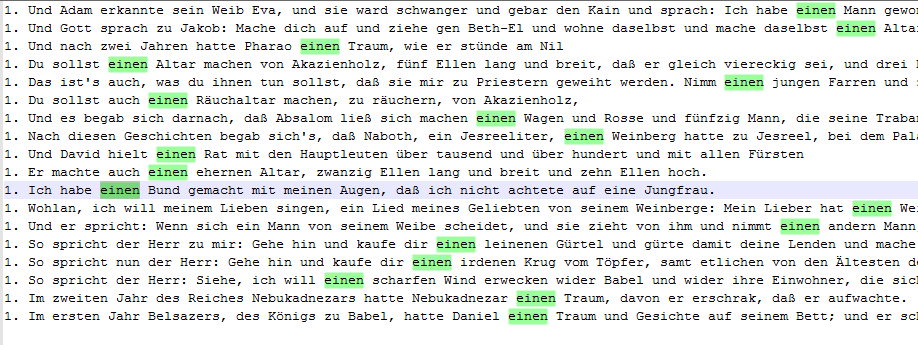
\includegraphics[width=1\textwidth]{Ingo/Bilder/SimpleKMeans100Attr1024Cluster_554.png}
\caption{100 Attribute, 1024 Cluster, Cluster 554}
\label{fig:100Attribute1024ClusterCluster554}
\end{figure}

\begin{figure}[htp]
\centering
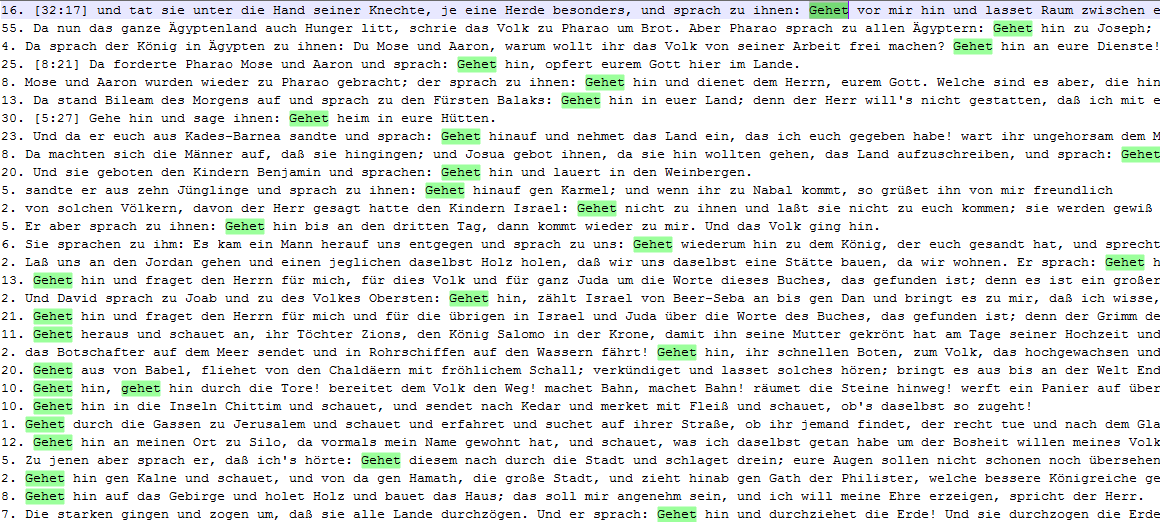
\includegraphics[width=1\textwidth]{Ingo/Bilder/SimpleKMeans1000Attr32Cluster_4.png}
\caption{1000 Attribute, 32 Cluster, Cluster 4}
\label{fig:1000Attribute32ClusterCluster4}
\end{figure}

\begin{figure}[htp]
\centering
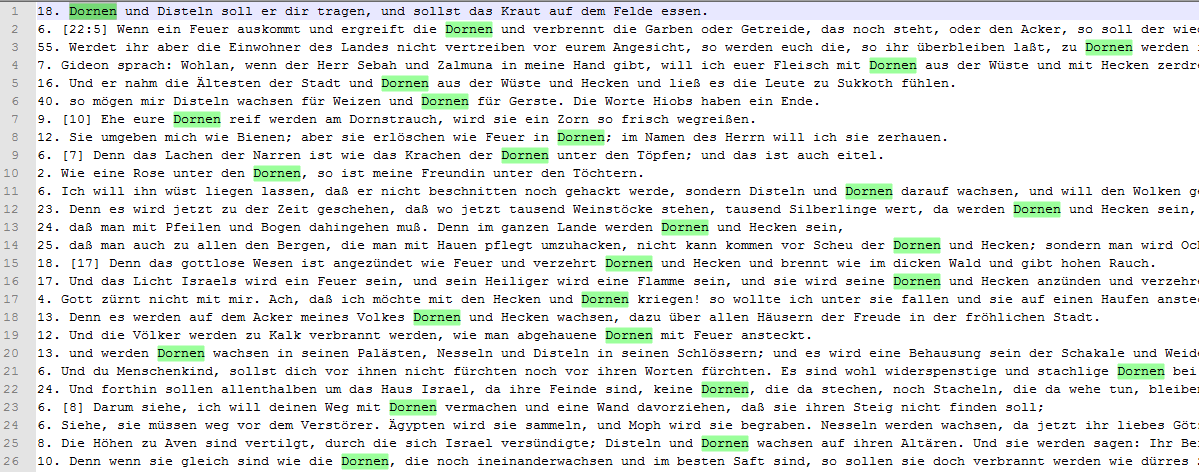
\includegraphics[width=1\textwidth]{Ingo/Bilder/SimpleKMeans1000Attr32Cluster_5.png}
\caption{1000 Attribute, 32 Cluster, Cluster 5}
\label{fig:1000Attribute32ClusterCluster5}
\end{figure}

\begin{figure}[htp]
\centering
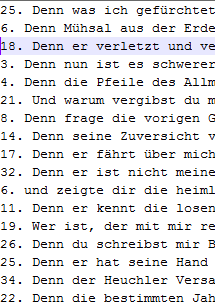
\includegraphics[width=1\textwidth]{Ingo/Bilder/SimpleKMeans1000Attr32Cluster_6.png}
\caption{1000 Attribute, 32 Cluster, Cluster 6}
\label{fig:1000Attribute32ClusterCluster6}
\end{figure}


\begin{figure}[htp]
\centering
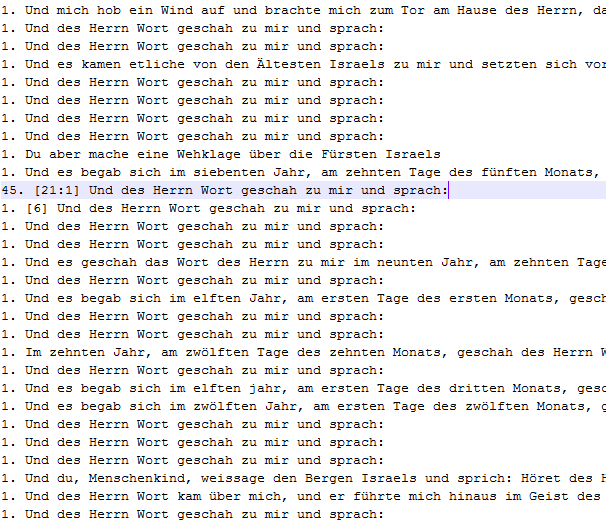
\includegraphics[width=1\textwidth]{Ingo/Bilder/SimpleKMeans1000Attr32Cluster_15.png}
\caption{1000 Attribute, 32 Cluster, Cluster 15}
\label{fig:1000Attribute32ClusterCluster15}
\end{figure}
